% ============================================================================
%  informe_desafio.tex - Informe final del proyecto (modalidad Desafío)
%  Electrónica Digital 1 - Universidad Nacional de Colombia, sede Bogotá
%  Juan David Ortiz Muñoz, David Eduardo Chivata Arias, Daniel Felipe Castro González
%  Compilar con: pdflatex informe_desafio.tex (dos veces, por las referencias)
% ============================================================================
\documentclass[conference,a4paper]{IEEEtran}
\usepackage[utf8]{inputenc}
\usepackage[T1]{fontenc}
\usepackage[spanish,es-noshorthands,es-tabla]{babel}
\usepackage{lmodern}
\usepackage{graphicx}
\usepackage{booktabs}
\usepackage{float}
\usepackage{tabularx}
\usepackage{array}
\usepackage{xcolor}
\usepackage{url}
\usepackage[hidelinks]{hyperref}
\usepackage{newunicodechar}
\newunicodechar{Ω}{\ensuremath{\Omega}}
\newunicodechar{→}{\ensuremath{\rightarrow}}
\graphicspath{{../figuras/}{../../fases/F4_interfaz_visual/}}
\newcolumntype{Y}{>{\raggedright\arraybackslash}X}
\newcommand{\ok}{\textcolor{green!45!black}{\textbf{Pasa}}}
\newcommand{\obs}{\textcolor{green!45!black}{\textbf{Observado}}}
\newcommand{\parcial}{\textcolor{orange!80!black}{\textbf{Parcial}}}

\begin{document}

% ============================================================================
% 1. Título
% ============================================================================
\title{Pong para dos jugadores en FPGA: implementación, pruebas y resultados}

\author{\IEEEauthorblockN{Juan David Ortiz Muñoz, David Eduardo Chivata Arias y Daniel Felipe Castro González}
\IEEEauthorblockA{Departamento de Ingeniería Eléctrica y Electrónica\\
Universidad Nacional de Colombia, sede Bogotá\\
\{juaortizmu, dchivata, dcastrogon\}@unal.edu.co}}

\maketitle

\begin{abstract}
Implementamos un videojuego Pong para dos jugadores usando solo lógica digital descrita en Verilog sobre una FPGA Cyclone~IV~E EP4CE10E22C8N. La FPGA calcula las posiciones de las paletas y de la pelota, detecta impactos y goles con lógica combinacional, controla el juego con una máquina de estados de seis estados, lleva el puntaje hasta nueve y dibuja el tablero de $8\times16$ LED en dos matrices con controlador compatible con MAX7219. El puntaje sale en BCD hacia dos decodificadores CD4511BE y dos displays de siete segmentos; todas las salidas pasan de 3,3~V a 5~V por dos búferes SN74HCT245N. Verificamos el diseño con 19 bancos de prueba (todos pasan) y en hardware con una partida completa hasta 9--6, victoria, RESET y nueva partida. Los controles inalámbricos de la propuesta se reemplazaron por mandos cableados con detección de conexión.
\end{abstract}

\begin{IEEEkeywords}
FPGA, Verilog, Pong, máquina de estados, MAX7219, CD4511BE, SN74HCT245N, verificación.
\end{IEEEkeywords}

% ============================================================================
% 2. Introducción
% ============================================================================
\section{Introducción}

El Pong es un buen pretexto para juntar casi todo lo que se ve en un curso de electrónica digital. Tiene entradas que hay que sincronizar y filtrar, posiciones que se guardan en registros y cambian con contadores, decisiones combinacionales (¿la pelota tocó la paleta o fue gol?), un control secuencial que decide en qué momento del juego estamos y una salida que exige un protocolo serial con tiempos precisos~\cite{mano,brown,tocci}. Nuestra propuesta fue hacerlo todo en una FPGA y sin microcontroladores, de modo que cada bloque tuviera que diseñarse con tablas de verdad, tablas de transición y máquinas de estados~\cite{propuesta}.

Los objetivos específicos de la propuesta eran: (1)~definir reglas, entradas, salidas y estados; (2)~diseñar los bloques con tablas y FSM; (3)~implementar en Verilog paletas, pelota, colisiones y puntaje; (4)~generar la imagen de $8\times16$ y la interfaz con los dos MAX7219; (5)~integrar dos controles inalámbricos; (6)~mostrar el puntaje en displays de siete segmentos; (7)~simular cada módulo y el conjunto; y (8)~implementar el prototipo y verificarlo en la FPGA.

Trabajamos por fases según nuestra guía metodológica~\cite{guia}: especificación (F0), arquitectura (F1), diseño lógico formal (F2), RTL y simulación (F3), pantalla (F4), controles (F5), marcador y montaje (F6) e informe del prototipo en protoboard (F7). Este informe describe la arquitectura implementada, las pruebas que hicimos, el uso que le dimos a herramientas de inteligencia artificial y las conclusiones. Todo el material (memorias de fase, código, bancos de prueba, reportes de Quartus y conexiones) está en el repositorio del proyecto~\cite{repo}.

% ============================================================================
% 3. Arquitectura implementada
% ============================================================================
\section{Arquitectura implementada}

\subsection{Visión general}

La Fig.~\ref{fig:sistema} muestra el sistema. La tarjeta A-C4E6E10 aporta la FPGA y el oscilador de 50~MHz. Los jugadores mueven su paleta con un mando cableado de tres líneas (UP, DOWN y DETECT) y el juego se maneja con tres pulsadores (START, PAUSE y RESET). La FPGA genera tres señales seriales para las matrices (DIN, CLK\_LED y LOAD), ocho bits BCD para el marcador y la señal HCT\_EN que habilita los búferes.

\begin{figure*}[!t]
  \centering
  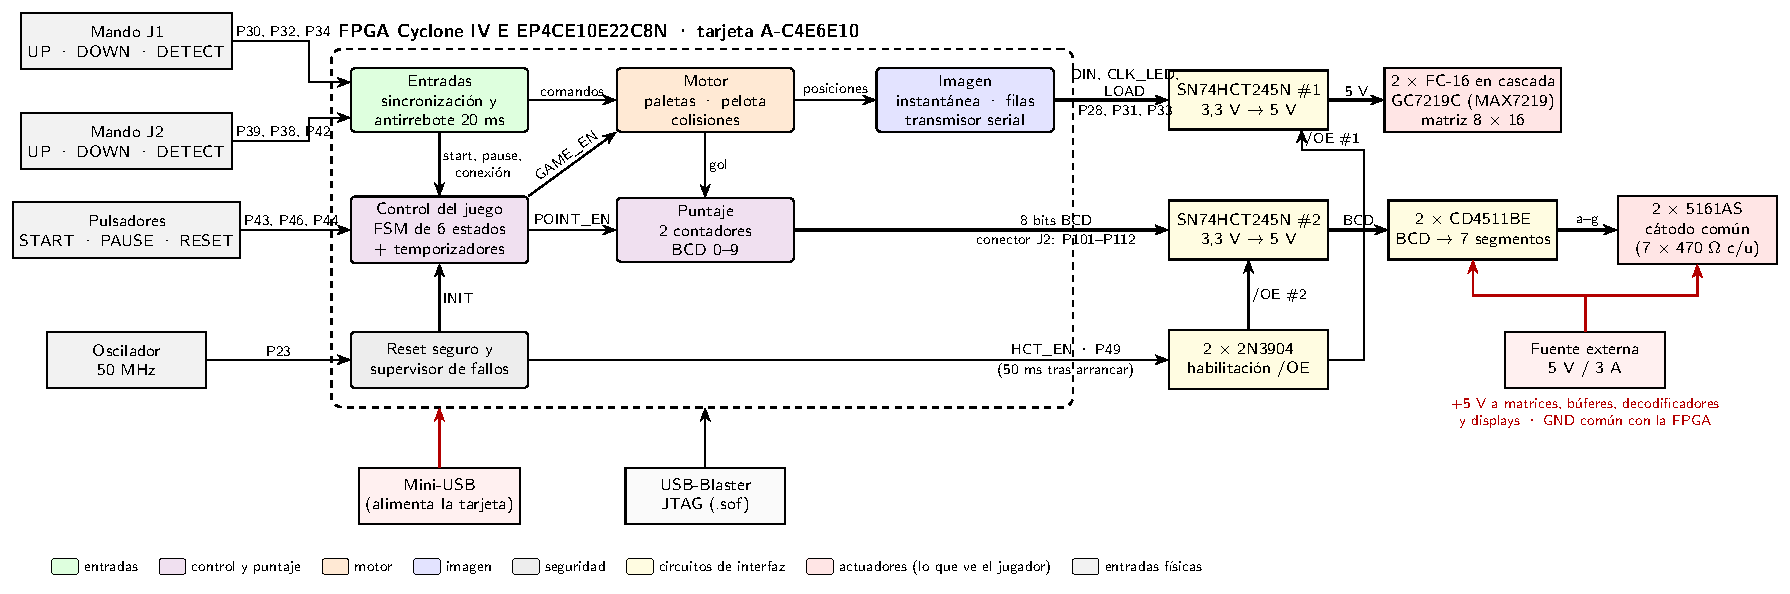
\includegraphics[width=\textwidth]{fig_sistema.pdf}
  \caption{Arquitectura del sistema implementado. A la izquierda las entradas físicas con sus pines; en el centro los bloques descritos en Verilog; a la derecha la interfaz de niveles y los actuadores.}
  \label{fig:sistema}
\end{figure*}

\subsection{Diseño digital en la FPGA}

La Fig.~\ref{fig:rtl} muestra cómo se conectan los módulos del núcleo. Todo el diseño usa un único reloj y avanza con pulsos de habilitación de un ciclo, no con relojes derivados, para evitar problemas de temporización.

\begin{figure*}[!t]
  \centering
  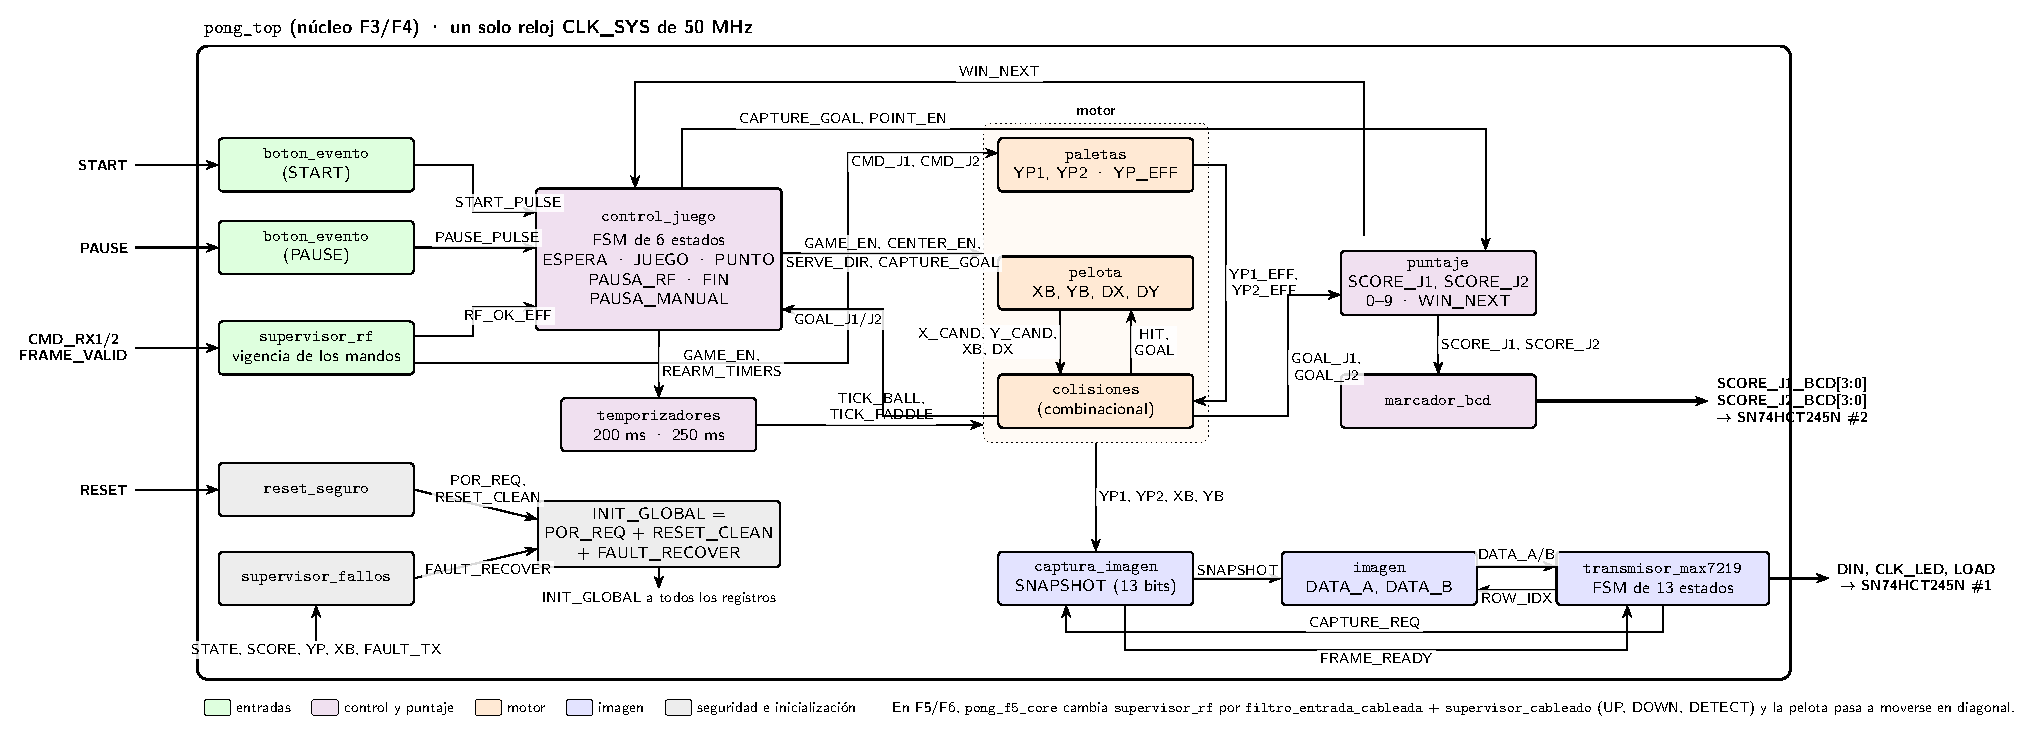
\includegraphics[width=\textwidth]{fig_rtl.pdf}
  \caption{Jerarquía del núcleo en Verilog con las señales principales entre módulos.}
  \label{fig:rtl}
\end{figure*}

\textbf{Entradas.} Cada entrada pasa por dos flip-flops de sincronización y un antirrebote de 20~ms ($10^6$ ciclos). START y PAUSE generan un pulso de un ciclo por pulsación. En la versión final cada mando entrega sus comandos de subir y bajar, y DETECT indica si está conectado; esa señal reemplaza la ``vigencia del enlace'' que en el diseño original venía del receptor RF.

\textbf{Control.} La FSM del juego (Fig.~\ref{fig:fsm}) tiene seis estados codificados en tres bits. En JUEGO las prioridades son: desconexión de un mando, luego PAUSE y luego gol. Al marcar un gol el sistema pasa por PUNTO, que suma una sola vez, y vuelve a ESPERA para un nuevo saque o va a FIN si el anotador llega a nueve. FIN solo se abandona con RESET. Dos temporizadores de 24 bits generan los pulsos de la pelota (200~ms) y de las paletas (250~ms).

\begin{figure}[!t]
  \centering
  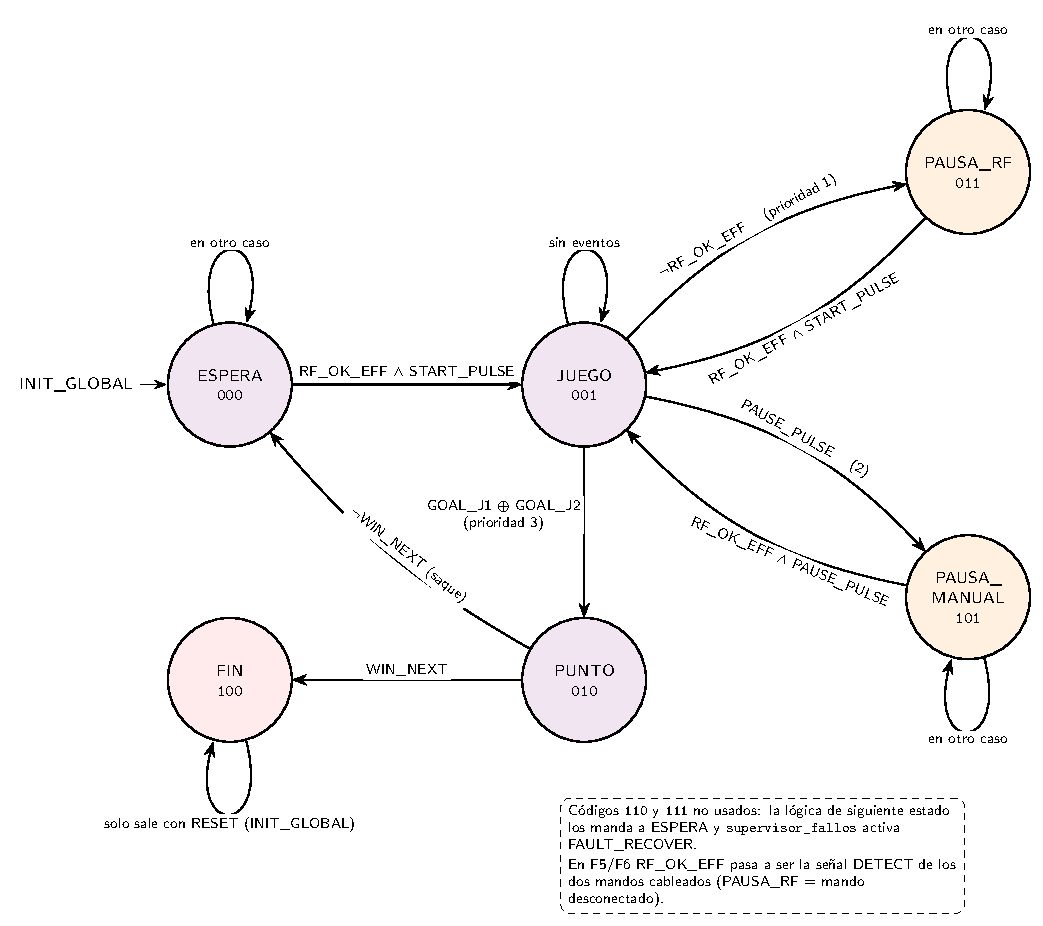
\includegraphics[width=\columnwidth]{fig_fsm.pdf}
  \caption{FSM de control del juego (\texttt{control\_juego.v}). INIT\_GLOBAL lleva a ESPERA desde cualquier estado.}
  \label{fig:fsm}
\end{figure}

\textbf{Motor.} Las paletas ocupan dos LED en las columnas 0 y 15 y se mueven entre las filas 0 y 6. La pelota tiene posición (XB, YB) y dirección (DX, DY); en la versión final avanza en diagonal en cada pulso. El módulo de colisiones es combinacional: con la posición candidata de la pelota y la posición efectiva de las paletas decide si hay rebote en pared, rebote en paleta (incluidas las esquinas) o gol.

\textbf{Puntaje.} Dos contadores de 0 a 9 que se incrementan con POINT\_EN según quién anotó. Las salidas ya están en BCD y van directo a los pines.

\textbf{Imagen.} Para que la pantalla nunca muestre un cuadro a medias, el módulo \texttt{captura\_imagen} toma una instantánea de 13 bits de las posiciones al comienzo de cada cuadro, con un intercambio CAPTURE\_REQ/FRAME\_READY con el transmisor. El módulo \texttt{imagen} arma combinacionalmente el byte de cada matriz para la fila pedida, y \texttt{transmisor\_max7219} es una FSM de 13 estados que primero envía las 14 instrucciones de configuración y luego refresca las ocho filas con tramas de 32 bits (16 para cada controlador de la cascada)~\cite{max7219}.

\textbf{Seguridad.} \texttt{reset\_seguro} genera un reset al encender y filtra el pulsador RESET. \texttt{supervisor\_fallos} revisa que el estado, el puntaje y las posiciones estén en rangos válidos; si encuentra un valor imposible activa FAULT\_RECOVER. Las tres causas se combinan en INIT\_GLOBAL, que reinicia todos los registros.

\subsection{Circuito externo}

La Fig.~\ref{fig:conexiones} es el circuito a nivel de pines. Los GPIO de la tarjeta están a 3,3~V~\cite{cyclone} y los periféricos a 5~V, así que usamos dos SN74HCT245N, cuyos umbrales de entrada TTL aceptan 3,3~V como uno lógico~\cite{hct245}. El /OE de cada búfer tiene pull-up a 5~V y un 2N3904 que lo pone en bajo cuando HCT\_EN sube (unos 50~ms después de configurar la FPGA); mientras tanto los búferes quedan en alta impedancia. Cada CD4511BE maneja un display 5161AS de cátodo común con siete resistencias de 470~Ω~\cite{cd4511,disp}. Los ocho bits BCD salen por el conector J2 (LCD) de la tarjeta, lo que obligó a configurar el pin~101 (nCEO) como E/S normal.

\begin{figure*}[!t]
  \centering
  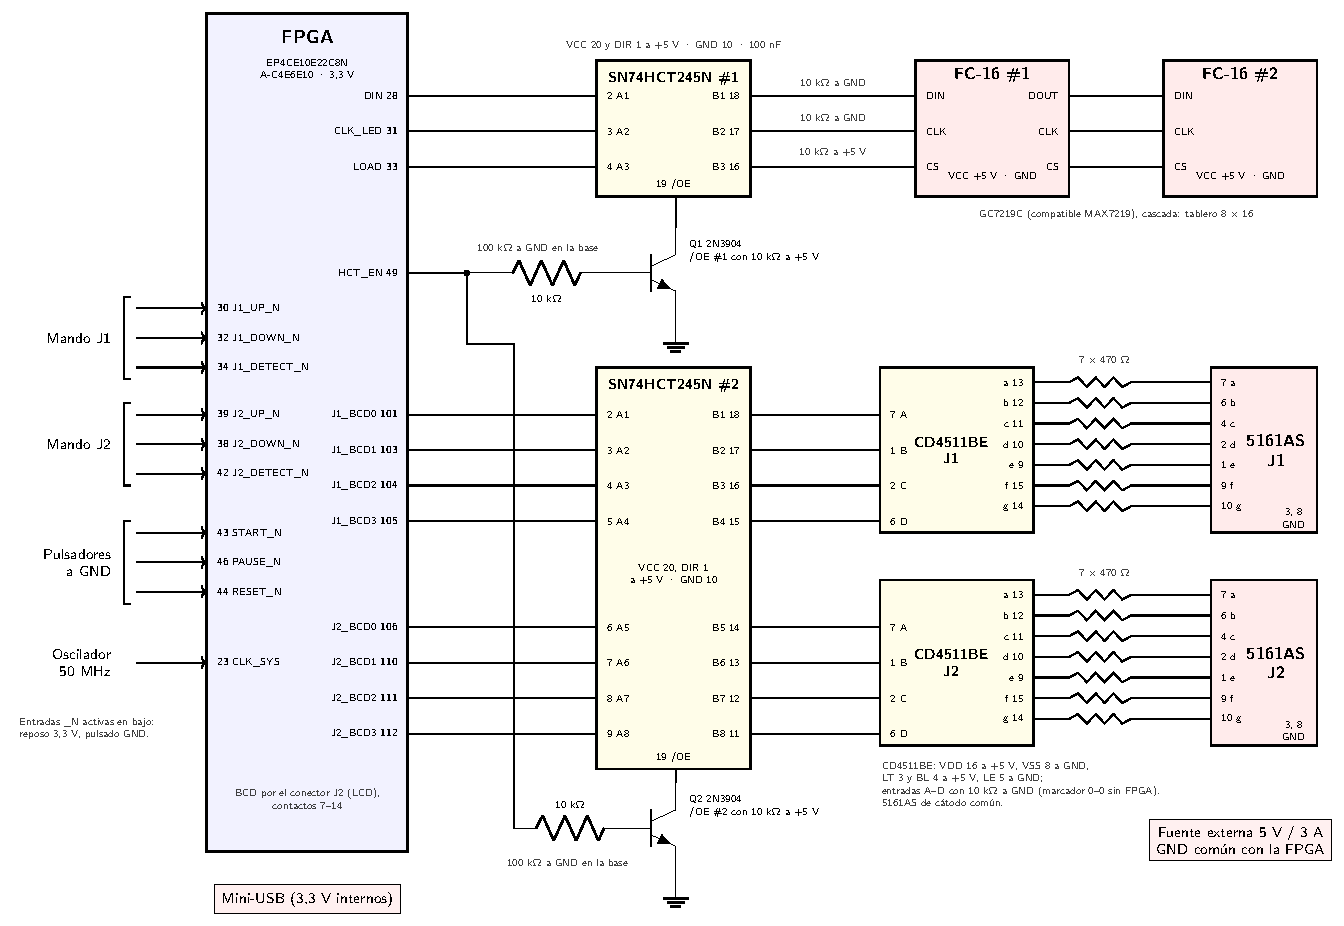
\includegraphics[width=0.94\textwidth]{fig_conexiones.pdf}
  \caption{Circuito de conexiones del prototipo con los números de pin de la FPGA y de cada integrado.}
  \label{fig:conexiones}
\end{figure*}

\subsection{Diferencias con la propuesta}

\begin{itemize}
\item \textbf{Controles cableados en lugar de inalámbricos.} No integramos módulos RF. Como la arquitectura ya aislaba el enlace en su propio módulo, el cambio se limitó a la entrada; la FSM y el estado PAUSA\_RF se mantuvieron, ahora activados por la desconexión de un mando. Esto deja el objetivo~5 cumplido solo en su lógica, no con radio.
\item \textbf{Movimiento diagonal de la pelota} (X e Y en cada pulso), en lugar de Y a la mitad de velocidad, porque en la matriz real el juego se veía lento.
\item \textbf{Dos SN74HCT245N} en lugar de un SN74AHCT125, porque había que adaptar once líneas.
\item \textbf{Orientación de las matrices.} En F4 corregimos el orden de bits y de filas para que coincidiera con los módulos FC-16 reales.
\end{itemize}

% ============================================================================
% 4. Pruebas
% ============================================================================
\section{Pruebas}

Probamos en tres niveles: simulación de cada módulo y del sistema, compilación y análisis de tiempos en Quartus, y pruebas físicas en la tarjeta.

\subsection{Simulación}

Para cada módulo escribimos un banco de prueba que compara la salida contra un modelo independiente, derivado de las tablas de F2. Cuando el espacio de entradas lo permitía, recorrimos todas las combinaciones válidas. Además hicimos cinco bancos de integración sobre \texttt{pong\_top} que reproducen situaciones de juego completas. La Tabla~\ref{tab:sim} resume los resultados. Las simulaciones se hicieron en Questa durante F3 y luego las repetimos con Icarus Verilog~\cite{icarus}; en el repositorio corren solas con cada cambio.

\begin{table*}[!t]
\centering
\caption{Resultados de simulación (19 de 19 pasan)}
\label{tab:sim}
\footnotesize
\begin{tabularx}{\textwidth}{@{}>{\raggedright\arraybackslash}p{0.36\textwidth} Y l@{}}
\toprule
\textbf{Banco de prueba} & \textbf{Qué se comprueba} & \textbf{Res.} \\
\midrule
\texttt{tb\_colisiones} & 87\,823 casos de bordes, paletas, esquinas y goles & \ok \\
\texttt{tb\_imagen} & 65\,546 combinaciones de posiciones y filas & \ok \\
\texttt{tb\_control\_juego} & 512 combinaciones de estado y entradas de la FSM & \ok \\
\texttt{tb\_supervisor\_fallos} & 363 comprobaciones de estados y registros inválidos & \ok \\
\texttt{tb\_marcador\_bcd} & 356 comprobaciones de los buses BCD & \ok \\
\texttt{tb\_reset\_seguro} & 47 comprobaciones de arranque y RESET & \ok \\
\texttt{tb\_pelota} & 39 casos de movimiento y rebote & \ok \\
\texttt{tb\_puntaje} & 37 casos de conteo y victoria & \ok \\
\texttt{tb\_paletas} & 14 casos de límites y comandos & \ok \\
\texttt{tb\_captura\_imagen} & 13 casos del intercambio de captura & \ok \\
\texttt{tb\_boton\_evento}, \texttt{tb\_temporizadores}, \texttt{tb\_supervisor\_rf}, \texttt{tb\_transmisor\_max7219} & Antirrebote, pulsos de 200/250~ms, vigencia del enlace, inicialización y tramas de 32 bits & \ok \\
\midrule
\texttt{tb\_pong\_integracion} & 9/9: arranque, saque y juego & \ok \\
\texttt{tb\_pong\_colisiones\_rebotes} & 8/8: rebotes en el sistema completo & \ok \\
\texttt{tb\_pong\_goles\_victoria} & 13/13: goles, puntaje y FIN & \ok \\
\texttt{tb\_pong\_recuperacion\_fallos} & 11/11: inyección de fallos y recuperación & \ok \\
\texttt{tb\_pong\_max7219\_integrado} & 8/8: tramas reales hacia la cascada & \ok \\
\bottomrule
\end{tabularx}
\end{table*}

Tres bancos (\texttt{tb\_imagen}, \texttt{tb\_transmisor\_max7219} y \texttt{tb\_pong\_max7219\_integrado}) tuvieron que actualizarse después de F4, porque la corrección de orientación cambió el orden de bits esperado. Comprobamos que con el código de F3 los bancos originales siguen pasando y que con el código corregido pasan los actualizados.

\subsection{Compilación y temporización}

La Tabla~\ref{tab:quartus} recoge las tres compilaciones de referencia en Quartus Prime 25.1 Lite. En todas el diseño cumple con el reloj de 50~MHz (periodo de 20~ns) y no hay rutas sin restricción. En F6 agregamos al archivo SDC un presupuesto provisional de retardo para las salidas BCD; los márgenes que se reportan dependen de esas suposiciones y no certifican los retardos reales de la protoboard.

\begin{table}[H]
\centering
\caption{Compilaciones en Quartus (EP4CE10E22C8)}
\label{tab:quartus}
\footnotesize
\begin{tabularx}{\columnwidth}{@{}Y c c c@{}}
\toprule
& \textbf{F3} & \textbf{F4} & \textbf{F6} \\
\midrule
Top & \texttt{pong\_top} & prueba visual & integración \\
Elementos lógicos & 560 & 160 & 660 \\
Registros & 276 & 80 & -- \\
Pines & 21 & 4 & 22 \\
Errores & 0 & 0 & 0 \\
\textit{Setup slack} (peor) & -- & $+11{,}112$~ns & $+6{,}686$~ns \\
\textit{Hold slack} (peor) & -- & $+0{,}187$~ns & $+0{,}186$~ns \\
\bottomrule
\end{tabularx}
\end{table}

Quedan ocho advertencias en la compilación final. La única que tiene que ver con el hardware es la 169177, sobre compatibilidad de las entradas LVTTL de 3,3~V; la dejamos documentada para revisarla con la nota AN~447~\cite{an447}.

\subsection{Pruebas físicas}

Las pruebas en la tarjeta se hicieron por etapas. En F4 programamos un top que solo maneja la pantalla y verificamos la posición inicial de paletas y pelota (Fig.~\ref{fig:f4}). En F5 probamos el juego con los mandos. En F6 montamos el marcador: primero aislado, forzando valores BCD a mano, y luego conectado a la FPGA. La Tabla~\ref{tab:fisicas} resume lo observado.

\begin{figure}[H]
  \centering
  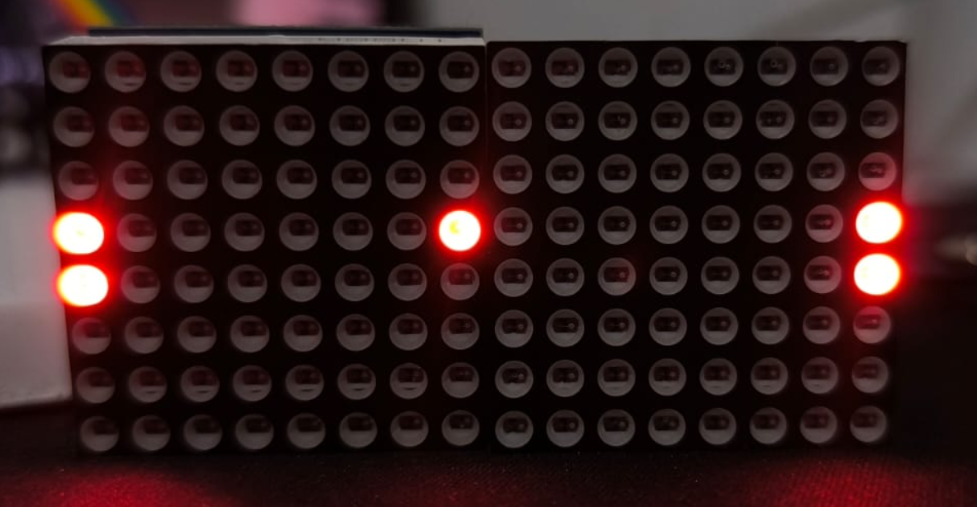
\includegraphics[width=0.9\columnwidth]{F4_Prueba_Visual_MAX7219.png}
  \caption{Prueba de F4: paletas en las columnas 0 y 15 y pelota en su posición inicial, en las dos matrices en cascada.}
  \label{fig:f4}
\end{figure}

\begin{table*}[!t]
\centering
\caption{Pruebas físicas sobre la tarjeta}
\label{tab:fisicas}
\footnotesize
\begin{tabularx}{\textwidth}{@{}l l Y l@{}}
\toprule
\textbf{Fase} & \textbf{Prueba} & \textbf{Resultado observado} & \textbf{Estado} \\
\midrule
F4 & Inicialización y cuadro inicial & Programación JTAG al 100~\%; las dos matrices muestran paletas y pelota en la posición esperada tras corregir la orientación & \obs \\
F5 & Paletas independientes & Cada mando mueve solo su paleta y se respetan los límites & \obs \\
F5 & START, PAUSE y RESET & Arranque, pausa y reanudación, y reinicio del juego & \obs \\
F5 & Movimiento y rebotes & Movimiento diagonal, rebotes en paredes y paletas, goles & \obs \\
F5 & Desconexión de un mando & El juego se detiene y no sigue mientras el mando está desconectado & \obs \\
F6 & Marcador aislado & Con BCD forzado, los displays muestran 0--0 y 1--0 & \obs \\
F6 & Búferes deshabilitados & Con HCT\_EN en bajo, los pull-down de los CD4511BE dejan 0--0 & \obs \\
F6 & Tensiones & 5,22~V en VCC del búfer~\#2 y 3,27~V en HCT\_EN con la FPGA configurada & Medido \\
F6 & Sistema completo & Matrices, dos búferes, dos decodificadores y dos displays funcionando a la vez & \obs \\
F6 & Partida completa & El puntaje sube en ambos jugadores hasta 9--6 y el juego se detiene en FIN & \obs \\
F6 & RESET y nueva partida & RESET devuelve el marcador a 0--0 y START inicia otra partida & \obs \\
F6 & Encendido y apagado & Con 5~V presentes y la FPGA sin configurar aparecen patrones transitorios & \parcial \\
\bottomrule
\end{tabularx}
\end{table*}

\subsection{Cumplimiento de los objetivos}

Con estas pruebas, los objetivos 1, 2, 3, 4, 6, 7 y 8 de la propuesta están cumplidos. El objetivo~5 está cumplido de forma parcial: los dos jugadores controlan sus paletas de manera independiente y el sistema reacciona a la pérdida de un mando, pero sin enlace inalámbrico. De los doce requisitos de F0, nueve están cumplidos y tres (R09 enlace, R10 revisión eléctrica y R12 prioridades del enlace) quedan parciales por la misma razón y por la advertencia de las entradas.

% ============================================================================
% 5. Uso de inteligencia artificial
% ============================================================================
\section{Uso de inteligencia artificial}

Usamos herramientas de IA en dos partes del proyecto y queremos dejarlo claro:

\begin{itemize}
\item \textbf{Durante las fases F0 a F7}, usamos asistentes de IA conversacionales para depurar y revisar: buscar la causa de errores de compilación y de simulación, revisar la redacción de las memorias y comprobar que tablas, ecuaciones y código fueran coherentes entre sí. Las especificaciones, el diseño lógico, el código Verilog, los bancos de prueba, el montaje, las mediciones y las pruebas en la tarjeta los hicimos nosotros.
\item \textbf{Organización del repositorio y estos informes.} Con Claude (Anthropic) organizamos el repositorio a partir de las entregas de cada fase; reprodujimos las simulaciones con Icarus Verilog y dejamos la prueba automática; ajustamos los tres bancos de prueba afectados por la corrección de orientación de F4; dibujamos las figuras de este informe a partir de nuestras tablas de conexión y de la FSM; y redactamos el borrador del informe de avance y de este informe, que después revisamos. También lo usamos para revisar el esquemático preliminar y para preparar la caja del juego.
\end{itemize}

En todos los casos revisamos el resultado contra nuestras memorias y contra el código. Los resultados numéricos de este informe salen de nuestros reportes de simulación y de Quartus, no de la herramienta.

% ============================================================================
% 6. Conclusiones
% ============================================================================
\section{Conclusiones}

\begin{itemize}
\item Logramos un Pong completo para dos jugadores hecho solo con lógica digital: el juego corre en la FPGA, se ve en las dos matrices y el marcador funciona en hardware, con una partida real hasta 9--6, victoria, RESET y nueva partida.
\item Hacer primero el diseño formal (tablas, ecuaciones y FSM) y escribir los bancos de prueba contra esas tablas valió la pena: los errores que aparecieron en el hardware no fueron de lógica, sino de supuestos físicos, como la orientación de las matrices o el pin nCEO.
\item Integrar por partes (pantalla, controles y marcador) y probar el marcador aislado antes de conectarlo nos permitió encontrar fallas sin poner en riesgo la tarjeta.
\item La adaptación de 3,3~V a 5~V con búferes HCT habilitados por transistor resolvió la interfaz, pero no resuelve los transitorios cuando la FPGA no está configurada; para eso haría falta supervisar la alimentación de 5~V.
\item La deuda principal frente a la propuesta es el enlace inalámbrico. La arquitectura lo deja preparado, porque bastaría conectar receptores que entreguen UP, DOWN y una señal de enlace activo. Quedan además el arranque autónomo desde la memoria de configuración, el registro en video de las pruebas y el diseño de las placas en KiCad.
\end{itemize}

% ============================================================================
% 7. Bibliografía
% ============================================================================
\begin{thebibliography}{99}
\bibitem{propuesta} J. D. Ortiz Muñoz, D. E. Chivata Arias y D. F. Castro González, ``Diseño e implementación de un videojuego Pong mediante electrónica digital con FPGA y controles inalámbricos,'' propuesta corregida, Electrónica Digital~1, Univ. Nacional de Colombia, 2026.
\bibitem{guia} J. D. Ortiz Muñoz, D. E. Chivata Arias y D. F. Castro González, ``Guía metodológica de diseño, simulación y validación del videojuego Pong con FPGA,'' documento del proyecto, 2026.
\bibitem{repo} Repositorio del proyecto ``pong-fpga-digital1'' (memorias F0--F7, código, pruebas y hardware). [En línea]. Disponible: \url{https://github.com/dcastrogon-coder/pong-fpga-digital1}
\bibitem{mano} M. M. Mano y M. D. Ciletti, \textit{Digital Design}, 5.ª ed. Upper Saddle River, NJ, EE.~UU.: Pearson, 2013.
\bibitem{brown} S. Brown y Z. Vranesic, \textit{Fundamentals of Digital Logic with Verilog Design}, 3.ª ed. Nueva York, NY, EE.~UU.: McGraw-Hill, 2014.
\bibitem{tocci} R. J. Tocci, N. S. Widmer y G. L. Moss, \textit{Digital Systems: Principles and Applications}, 11.ª ed. Upper Saddle River, NJ, EE.~UU.: Pearson, 2011.
\bibitem{cyclone} Intel/Altera, \textit{Cyclone IV Device Handbook}, vol.~1, 2016.
\bibitem{an447} Intel/Altera, ``AN 447: Interfacing Cyclone III and Cyclone IV Devices with 3.3/3.0/2.5-V LVTTL/LVCMOS I/O Systems,'' nota de aplicación.
\bibitem{max7219} Analog Devices/Maxim Integrated, ``MAX7219/MAX7221: Serially interfaced, 8-digit LED display drivers,'' hoja de datos, rev.~6, 2021.
\bibitem{hct245} Texas Instruments, ``SN74HCT245: Octal bus transceivers with 3-state outputs,'' hoja de datos. [En línea]. Disponible: \url{https://www.ti.com/product/SN74HCT245}
\bibitem{cd4511} Texas Instruments, ``CD4511B CMOS BCD-to-7-segment latch decoder drivers,'' hoja de datos SCHS072B. [En línea]. Disponible: \url{https://www.ti.com/lit/ds/symlink/cd4511b.pdf}
\bibitem{disp} Shanghai Toplite Technology, ``TOP-CC-5161AS: Seven-segment display,'' hoja de datos, 2014.
\bibitem{icarus} S. Williams, ``Icarus Verilog.'' [En línea]. Disponible: \url{https://steveicarus.github.io/iverilog/}
\end{thebibliography}

\end{document}
